\chapter{Systems} \label{chp:systems}
\epigraph{We must be clear that when it comes to atoms, language can be used only as in poetry.}{Niels Bohr}
\begin{figure}[H]
	\centering
	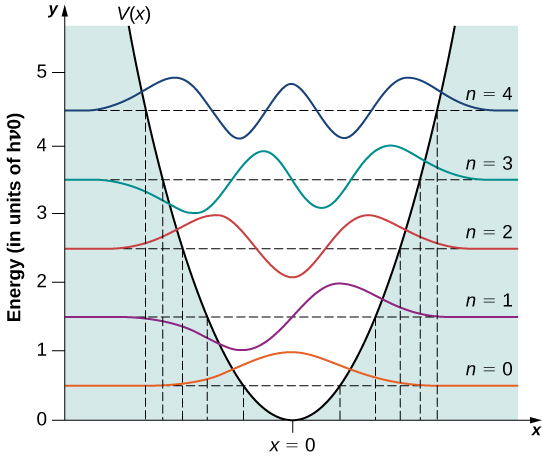
\includegraphics[scale=0.9]{Images/qho.jpg}
	\caption{The quantum harmonic oscillator, with the Hermite functions represented up to 4th order. As in classical mechanics, the harmonic oscillator can describe various quantum systems, such as lattice vibration (phonons) and quantum fields.}
	\label{fig:harmonicoscillator}
\end{figure}

When defining a system, we also need to specify the basis set to be used. The single particle functions are often known, and they are well-suited as a basis for the total

\newpage
\section{Quantum dots} \label{subsubsec:quantumdots}
Quantum dots are very small particles, and contain fermions or bosons hold together by an external potential. Since these particles have discrete electronic states like an atom, they are often called artificial atoms. 

In this thesis we will study electrons trapped in harmonic oscillators, where the external potential affecting particle $i$ is given by
\begin{equation}
u_i=\frac{1}{2}m\omega^2r_i^2.
\end{equation}
Using natural units as described in Appendix B, we can write the Hamiltonian as
\begin{equation}
\label{eq:HOHamiltonian}
\hat{\mathcal{H}} = \sum_{i=1}^{P} \Big(-\frac{1}{2} \nabla_i^2 + \frac{1}{2} r_i ^2\Big) + \sum_{i<j} \frac{1}{r_{ij}} 
\end{equation}
where the energy is scaled with respect to atomic units and lengths are scaled with respect to the Bohr radius.

The exact solutions of the non-interacting Hamiltonian are the Hermite functions, 
\begin{equation}
f_n(x)=H_n(x)\exp(-x^2/2)
\end{equation}
which form our basis. $H_n(x)$ is the Hermite polynomial of $n$'th degree, and the first four Hermite functions are illustrated in figure \eqref{fig:harmonicoscillator}.

We will study closed-shell systems only, since the Slater determinant in that case is unambiguous. For open shells, the total Slater determinant is a linear combination of all the possible Slater determinants. The number of particles of closed-shell systems are called magic numbers, which in two dimensions are $N=2,6,12,\hdots$. In general, the magic numbers are given by
\begin{equation}
N=s\binom{n+d}{d}
\end{equation}
where $s$ is the number of spin configurations (2), $n$ is the principal quantum number and $d$ is the number of dimensions. This is a direct consequence of the Pauli principle, where we in the ground state can have two particles with radial wave functions $\Phi_{n_x=0,n_y=0}$, in the next energy level we have have 4 particles with radial wave functions $\Phi_{n_x=1,n_y=0}$ and $\Phi_{n_x=0,n_y=1}$ with degeneracy 2 and so on. 

\section{Atomic systems} \label{subsubsec:atomic}
We will also investigate real atoms, where we freeze out the nucleonic degrees of freedom known as the Born-Oppenheimer approximation. The electrons will in fact affect the nucleus, but due to the mass difference this effect will be negligible.

We again have Coulomb interaction between the electrons and the nucleus, and since we assume it to be at rest at the origin, the external potential affecting particle $i$ is
\begin{equation}
u_i=- \frac{1}{2} k\frac{Ze^2}{r_i},
\end{equation}
where $Z$ is the atomic number (number of protons in the nucleus). The total Hamiltonian is given in (Hartree) atomic units, 
\begin{equation}
\label{eq:AtomicHamiltonian}
\hat{\mathcal{H}} = \sum_{i=1}^{P} \Big(-\frac{1}{2} \nabla_i^2 - \frac{1}{2} \frac{Z}{r_i}\Big) + \sum_{i<j} \frac{1}{r_{ij}},
\end{equation}
which also is discussed in Appendix B. 

"Colloquially, we call such solutions and derived properties as electronic structure."

\section{Molecular systems}

\section{Bose-Einstein Condensation}

\section{Electron gas} \label{subsubsec:electrongas}
\section{Helium gas} \label{subsubsec:heliumgas}
He$^3$ and He$^4$